	\paragraph{QuizziPedia::Front-End::Directives::ClickableAnswerDirective}
		
		\label{QuizziPedia::Front-End::Directives::ClickableAnswerDirective}
		
		\begin{figure}[ht]
			\centering
			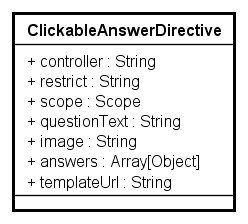
\includegraphics[scale=0.5,keepaspectratio]{UML/Classi/Front-End/QuizziPedia_Front-end_Templates_ClickableAnswerTemplate.png}
			\caption{QuizziPedia::Front-End::Directives::ClickableAnswerTemplate}
		\end{figure} \FloatBarrier
		
		\begin{itemize}
			\item \textbf{Descrizione}: rappresenta il componente grafico che permette all'utente di visualizzare la domanda ad area cliccabile nell'immagine. Viene visualizzato dinamicamente all'interno delle views TrainingView e FillingQuestionnaireView mediante il controller QuestionsController;
			\item \textbf{Utilizzo}: viene utilizzato per consentire all'utente la compilazione della domanda ad area cliccabile nell'immagine;
			\item \textbf{Relazioni con altre classi}: 
			\begin{itemize}
				\item \textit{IN} \texttt{TrainingView}: view principale della modalità allenamento; 
				\item \textit{IN} \texttt{FillingQuestionnaireView}: view principale per la compilazione del questionario;
				\item \textit{IN} \texttt{QuestionsController}: questa classe permette di gestire il recupero delle domande per poterle stampare nella modalità allenamento;
				
			\end{itemize}
			\item \textbf{Attributi}: 
			\begin{itemize}
				\item ;
			\end{itemize}
			\item \textbf{Metodi}: 
			\begin{itemize}
				\item ;
			\end{itemize}
		\end{itemize}
	
		\paragraph{QuizziPedia::Front-End::Directives::EmptySpaceAnswerDirective}
		
		\label{QuizziPedia::Front-End::Directives::EmptySpaceAnswerDirective}
		
		\begin{figure}[ht]
			\centering
			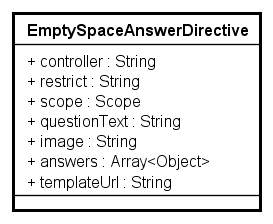
\includegraphics[scale=0.5,keepaspectratio]{UML/Classi/Front-End/QuizziPedia_Front-end_Templates_EmptySpaceAnswerTemplate.png}
			\caption{QuizziPedia::Front-End::Directives::EmptyChoiceAnswerDirective}
		\end{figure} \FloatBarrier
		
		\begin{itemize}
			\item \textbf{Descrizione}: rappresenta il componente grafico che permette all'utente di visualizzare l'esercizio a riempimento di spazi vuoti. Viene visualizzato dinamicamente all'interno delle views TrainingView e FillingQuestionnaireView mediante il controller QuestionsController;
			\item \textbf{Utilizzo}: viene utilizzato per consentire all'utente la compilazione dell'esercizio a riempimento di spazi vuoti;
			\item \textbf{Relazioni con altre classi}: 
			\begin{itemize}
				\item \textit{IN} \texttt{TrainingView}: view principale della modalità allenamento; 
				\item \textit{IN} \texttt{FillingQuestionnaireView}: view principale per la compilazione del questionario;
				\item \textit{IN} \texttt{QuestionsController}: questa classe permette di gestire il recupero delle domande per poterle stampare nella modalità allenamento;
			\end{itemize}
			\item \textbf{Attributi}: 
			\begin{itemize}
				\item ;
			\end{itemize}
			\item \textbf{Metodi}: 
			\begin{itemize}
				\item ;
			\end{itemize}
		\end{itemize}
		
		\paragraph{QuizziPedia::Front-End::Directives::HeaderTextQuestionDirective}
		
		\label{QuizziPedia::Front-End::Directives::HeaderTextQuestionDirective}
		
		\begin{figure}[ht]
			\centering
			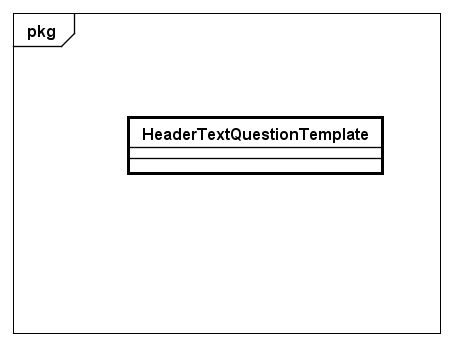
\includegraphics[scale=0.5,keepaspectratio]{UML/Classi/Front-End/QuizziPedia_Front-end_Templates_HeaderTextQuestionTemplate.png}
			\caption{QuizziPedia::Front-End::Directives::HeaderTextQuestionDirective}
		\end{figure} \FloatBarrier
		
		\begin{itemize}
			\item \textbf{Descrizione}: rappresenta il componente grafico che presenta all'utente il testo della domanda, l'argomento e le parole chiave. Viene visualizzato dinamicamente all'interno delle views TrainingView e FillingQuestionnaireView mediante il controller QuestionsController;
			\item \textbf{Utilizzo}: viene utilizzato per consentire all'utente la visualizzazione del testo della domanda, dell'argomento della domanda e le parole chiave associate ad essa;
			\item \textbf{Relazioni con altre classi}: 
			\begin{itemize}
				\item \textit{IN} \texttt{TrainingModelView}: ; 
				\item \textit{IN} \texttt{FillingQuestionnaireModelView}: ;
				\item \textit{IN} \texttt{QuestionsController}: questa classe permette di gestire il recupero delle domande per poterle stampare nella modalità allenamento;
			\end{itemize}
			\item \textbf{Attributi}: 
			\begin{itemize}
				\item ;
			\end{itemize}
			\item \textbf{Metodi}: 
			\begin{itemize}
				\item ;
			\end{itemize}
		\end{itemize}
		
		\paragraph{QuizziPedia::Front-End::Directives::InfoQuestionnaireDirective}
		
		\label{QuizziPedia::Front-End::Directives::InfoQuestionnaireDirective}
		
		\begin{figure}[ht]
			\centering
			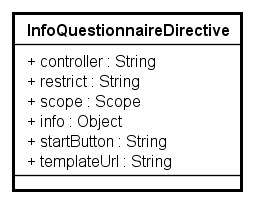
\includegraphics[scale=0.5,keepaspectratio]{UML/Classi/Front-End/QuizziPedia_Front-end_Templates_InfoQuestionnaireTemplate.png}
			\caption{QuizziPedia::Front-End::Directives::InfoQuestionnaireDirective}
		\end{figure} \FloatBarrier
		
		\begin{itemize}
			\item \textbf{Descrizione}: rappresenta il componente grafico che permette all'utente di visualizzare le informazioni principali del questionario che si sta per svolgere. Viene visualizzato dinamicamente all'interno della view FillingQuestionnaireView mediante il controller FillingQuestionsController;
			\item \textbf{Utilizzo}: viene utilizzato per consentire all'utente di visualizzare le informazioni principali del questionario che si sta per svolgere. Informazioni come:
			\begin{itemize}
				\item Nome del questionario;
				\item Nome dell'autore del questionario;
				\item Data di creazione del questionario;
				\item Argomento del questionario;
				\item Bottone per iniziare il questionario;
			\end{itemize}
			\item \textbf{Relazioni con altre classi}: 
			\begin{itemize}
				\item \textit{IN} \texttt{FillingQuestionnaireModelView}: view principale per la compilazione del questionario;
				\item \textit{IN} \texttt{FillingQuestionsController}: questa classe permette di gestire la creazione e la modifica di una domanda a riempimento di spazi;
			\end{itemize}
			\item \textbf{Attributi}: 
			\begin{itemize}
				\item ;
			\end{itemize}
			\item \textbf{Metodi}: 
			\begin{itemize}
				\item ;
			\end{itemize}
		\end{itemize}
		
		\paragraph{QuizziPedia::Front-End::Directives::LinkingAnswerDirective}
		
		\label{QuizziPedia::Front-End::Directives::LinkingAnswerDirective}
		
		\begin{figure}[ht]
			\centering
			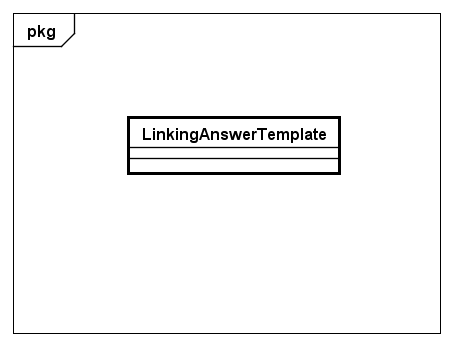
\includegraphics[scale=0.5,keepaspectratio]{UML/Classi/Front-End/QuizziPedia_Front-end_Templates_LinkingAnswerTemplate.png}
			\caption{QuizziPedia::Front-End::Directives::LinkingAnswerDirective}
		\end{figure} \FloatBarrier		
		
		\begin{itemize}
			\item \textbf{Descrizione}: rappresenta il componente grafico che permette all'utente di visualizzare la domanda di collegamento. Viene visualizzato dinamicamente all'interno delle views TrainingView e FillingQuestionnaireView mediante il controller QuestionsController;
			\item \textbf{Utilizzo}: viene utilizzato per consentire all'utente la compilazione della domanda di collegamento;
			\item \textbf{Relazioni con altre classi}: 
			\begin{itemize}
				\item \textit{IN} \texttt{TrainingModelView}: ; 
				\item \textit{IN} \texttt{FillingQuestionnaireModelView}: ;
				\item \textit{IN} \texttt{QuestionsController}: questa classe permette di gestire il recupero delle domande per poterle stampare nella modalità allenamento;
			\end{itemize}
			\item \textbf{Attributi}: 
			\begin{itemize}
				\item ;
			\end{itemize}
			\item \textbf{Metodi}: 
			\begin{itemize}
				\item ;
			\end{itemize}
		\end{itemize}
		
		\paragraph{QuizziPedia::Front-End::Directives::MultipleChoiceAnswerDirective}
		
		\label{QuizziPedia::Front-End::Directives::MultipleChoiceAnswerDirective}
		
		\begin{figure}[ht]
			\centering
			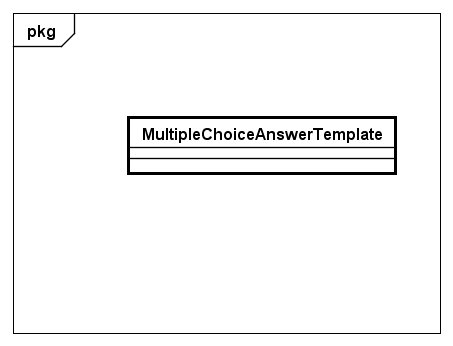
\includegraphics[scale=0.5,keepaspectratio]{UML/Classi/Front-End/QuizziPedia_Front-end_Templates_MultipleChoiceAnswerTemplate.png}
			\caption{QuizziPedia::Front-End::Directives::MultipleChoiceAnswerDirective}
		\end{figure} \FloatBarrier
		
		\begin{itemize}
			\item \textbf{Descrizione}: rappresenta il componente grafico che permette all'utente di visualizzare la domanda a risposta multipla. Viene visualizzato dinamicamente all'interno delle views TrainingView e FillingQuestionnaireView mediante il controller QuestionsController;
			\item \textbf{Utilizzo}: viene utilizzato per consentire all'utente la compilazione della domanda a risposta multipla;
			\item \textbf{Relazioni con altre classi}: 
			\begin{itemize}
				\item \textit{IN} \texttt{TrainingModelView}: ; 
				\item \textit{IN} \texttt{FillingQuestionnaireModelView}: ;
				\item \textit{IN} \texttt{QuestionsController}: questa classe permette di gestire il recupero delle domande per poterle stampare nella modalità allenamento;
				\item \textit{IN} \texttt{RightDirectiveModel}: ;
			\end{itemize}
			\item \textbf{Attributi}: 
			\begin{itemize}
				\item \texttt{QuestionText}: identifica il testo della domanda;
				\item \texttt{url}: identifica l'url di una possibile immagine nel testo della domanda;
				\item \texttt{Answer}: array che contiene coppie di valori. Queste coppie sono formate da:
				\begin{itemize}
					\item \texttt{Text}: contiene il testo dell'affermazione;
					\item \texttt{url}: identifica l'url di una possibile immagine nel testo della domanda;
					\item \texttt{isItRight}: contiene se la risposta è vero o falso.
				\end{itemize}
			\end{itemize}
			 
			\item \textbf{Metodi}: 
			\begin{itemize}
				\item ;
			\end{itemize}
		\end{itemize}
		
		\paragraph{QuizziPedia::Front-End::Directives::SortImagesAnswerDirective}
		
		\label{QuizziPedia::Front-End::Directives::SortImagesAnswerDirective}
		
		\begin{figure}[ht]
			\centering
			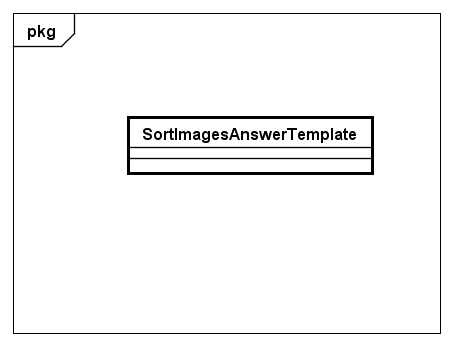
\includegraphics[scale=0.5,keepaspectratio]{UML/Classi/Front-End/QuizziPedia_Front-end_Templates_SortImagesAnswerTemplate.png}
			\caption{QuizziPedia::Front-End::Directives::SortImagesAnswerDirective}
		\end{figure} \FloatBarrier
		
		\begin{itemize}
			\item \textbf{Descrizione}: rappresenta il componente grafico che permette all'utente di visualizzare la domanda ad ordinamento di immagini. Viene visualizzato dinamicamente all'interno delle views TrainingView e FillingQuestionnaireView mediante il controller QuestionsController;
			\item \textbf{Utilizzo}: viene utilizzato per consentire all'utente la compilazione della domanda ad ordinamento di immagini;
			\item \textbf{Relazioni con altre classi}: 
			\begin{itemize}
				\item \textit{IN} \texttt{TrainingModelView}: ; 
				\item \textit{IN} \texttt{FillingQuestionnaireModelView}: ;
				\item \textit{IN} \texttt{QuestionsController}: questa classe permette di gestire il recupero delle domande per poterle stampare nella modalità allenamento;
			\end{itemize}
			\item \textbf{Attributi}: 
			\begin{itemize}
				\item ;
			\end{itemize}
			\item \textbf{Metodi}: 
			\begin{itemize}
				\item ;
			\end{itemize}
		\end{itemize}
		
		\paragraph{QuizziPedia::Front-End::Directives::SortTextAnswerDirective}
		
		\label{QuizziPedia::Front-End::Directives::SortTextAnswerDirective}
		
		\begin{figure}[ht]
			\centering
			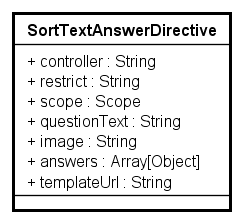
\includegraphics[scale=0.5,keepaspectratio]{UML/Classi/Front-End/QuizziPedia_Front-end_Templates_SortTextAnswerTemplate.png}
			\caption{QuizziPedia::Front-End::Directives::SortTextAnswerDirective}
		\end{figure} \FloatBarrier
		
		\begin{itemize}
			\item \textbf{Descrizione}: rappresenta il componente grafico che permette all'utente di visualizzare la domanda ad ordinamento di stringhe. Viene visualizzato dinamicamente all'interno delle views TrainingView e FillingQuestionnaireView mediante il controller QuestionsController;
			\item \textbf{Utilizzo}: viene utilizzato per consentire all'utente la compilazione della domanda ad ordinamento di stringhe;
			\item \textbf{Relazioni con altre classi}: 
			\begin{itemize}
				\item \textit{IN} \texttt{TrainingModelView}: ; 
				\item \textit{IN} \texttt{FillingQuestionnaireModelView}: ;
				\item \textit{IN} \texttt{QuestionsController}: questa classe permette di gestire il recupero delle domande per poterle stampare nella modalità allenamento;
			\end{itemize}
			\item \textbf{Attributi}: 
			\begin{itemize}
				\item ;
			\end{itemize}
			\item \textbf{Metodi}: 
			\begin{itemize}
				\item ;
			\end{itemize}
		\end{itemize}
		
		\paragraph{QuizziPedia::Front-End::Directives::TrainingSetUpDirective}
		
		\label{QuizziPedia::Front-End::Directives::TrainingSetUpDirective}
		
		\begin{figure}[ht]
			\centering
			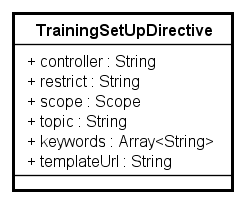
\includegraphics[scale=0.5,keepaspectratio]{UML/Classi/Front-End/QuizziPedia_Front-end_Templates_TrainingSetUpTemplate.png}
			\caption{QuizziPedia::Front-End::Directives::TrainingSetUpDirective}
		\end{figure} \FloatBarrier
		
		\begin{itemize}
			\item \textbf{Descrizione}: rappresenta il componente grafico che permette all'utente di selezionare l'argomento e le parole chiave per iniziare un allenamento con queste caratteristiche. Viene visualizzato dinamicamente all'interno della view TrainingView mediante il controller TrainingController;
			\item \textbf{Utilizzo}: viene utilizzato per consentire all'utente di selezionare l'argomento e le parole chiave di un allenamento;
			\item \textbf{Relazioni con altre classi}: 
			\begin{itemize}
				\item \textit{IN} \texttt{TrainingModelView}: ; 
				\item \textit{OUT} \texttt{TrainingController}: questa classe permette di gestire la modalità allenamento sottoponendo all'utente le giuste domande adatte al suo livello;
			\end{itemize}
			\item \textbf{Attributi}: 
			\begin{itemize}
				\item ;
			\end{itemize}
			\item \textbf{Metodi}: 
			\begin{itemize}
				\item ;
			\end{itemize}
		\end{itemize}
		
		\paragraph{QuizziPedia::Front-End::Directives::TrueFalseAnswerDirective}
		
		\label{QuizziPedia::Front-End::Directives::TrueFalseAnswerDirective}
		
		\begin{figure}[ht]
			\centering
			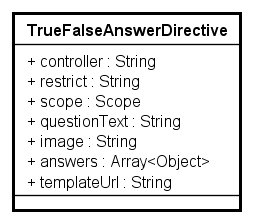
\includegraphics[scale=0.5,keepaspectratio]{UML/Classi/Front-End/QuizziPedia_Front-end_Templates_TrueFalseAnswerTemplate.png}
			\caption{QuizziPedia::Front-End::Directives::TrueFalseAnswerDirective}
		\end{figure} \FloatBarrier
		
		\begin{itemize}
			\item \textbf{Descrizione}: rappresenta il componente grafico che permette all'utente di visualizzare la domanda vero e falso. Viene visualizzato dinamicamente all'interno delle views TrainingView e FillingQuestionnaireView mediante il controller QuestionsController;
			\item \textbf{Utilizzo}: viene utilizzato per consentire all'utente la compilazione della domanda vero e falso;
			\item \textbf{Relazioni con altre classi}: 
			\begin{itemize}
				\item \textit{IN} \texttt{TrainingModelView}: ; 
				\item \textit{IN} \texttt{QuestionsController}: questa classe permette di gestire il recupero delle domande per poterle stampare nella modalità allenamento;
				\item \textit{IN} \texttt{RightDirectiveModel}: ;
			\end{itemize}
			\item \textbf{Attributi}: 
			\begin{itemize}
				\item \texttt{image}: identifica una possibile immagine nella domanda;
				\item \texttt{Answer}: array che contiene coppie di valori. Queste coppie sono formate da:
				\begin{itemize}
					\item \texttt{Text}: contiene il testo dell'affermazione;
					\item \texttt{isItRight}: contiene se la risposta è vero o falso.
				\end{itemize}
			\end{itemize}
			\item \textbf{Metodi}: 
			\begin{itemize}
				\item ;
			\end{itemize}
		\end{itemize}																	